% Recursion tree of T(n)=3T(n/2)+f(n) (generated by figs_c2ch01.py).
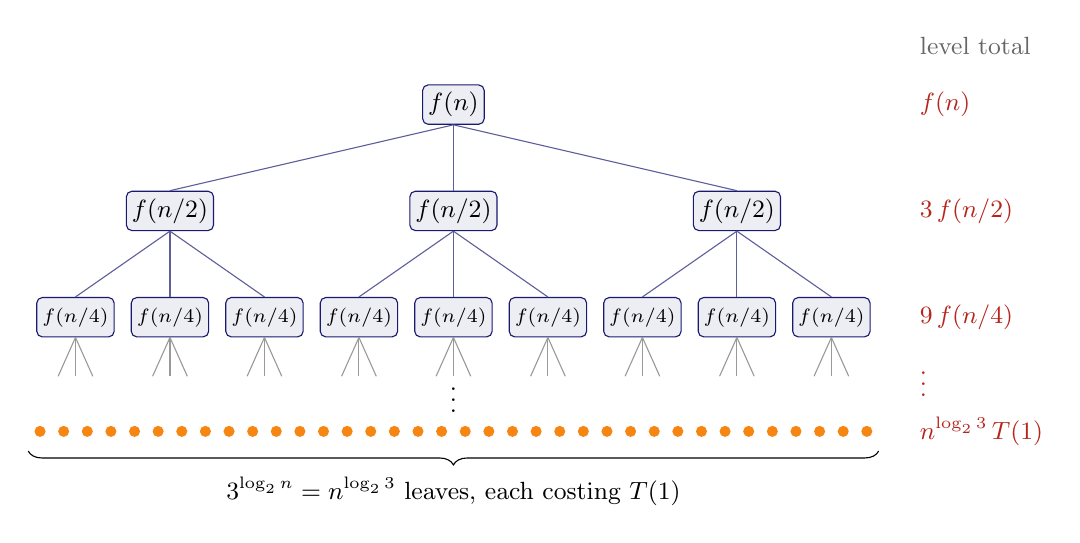
\begin{tikzpicture}[x=1cm,y=1cm,every node/.style={font=\small}]
\tikzset{nd/.style={draw=MidnightBlue,fill=MidnightBlue!8,rounded corners=2pt,inner sep=2pt,minimum height=0.5cm}}
\node[nd,font=\small] (n0_0) at (5.400,-0.00) {$f(n)$};
\node[nd,font=\small] (n1_0) at (1.800,-1.35) {$f(n/2)$};
\draw[MidnightBlue!70] (n0_0.south) -- (n1_0.north);
\node[nd,font=\small] (n1_1) at (5.400,-1.35) {$f(n/2)$};
\draw[MidnightBlue!70] (n0_0.south) -- (n1_1.north);
\node[nd,font=\small] (n1_2) at (9.000,-1.35) {$f(n/2)$};
\draw[MidnightBlue!70] (n0_0.south) -- (n1_2.north);
\node[nd,font=\scriptsize] (n2_0) at (0.600,-2.70) {$f(n/4)$};
\draw[MidnightBlue!70] (n1_0.south) -- (n2_0.north);
\node[nd,font=\scriptsize] (n2_1) at (1.800,-2.70) {$f(n/4)$};
\draw[MidnightBlue!70] (n1_0.south) -- (n2_1.north);
\node[nd,font=\scriptsize] (n2_2) at (3.000,-2.70) {$f(n/4)$};
\draw[MidnightBlue!70] (n1_0.south) -- (n2_2.north);
\node[nd,font=\scriptsize] (n2_3) at (4.200,-2.70) {$f(n/4)$};
\draw[MidnightBlue!70] (n1_1.south) -- (n2_3.north);
\node[nd,font=\scriptsize] (n2_4) at (5.400,-2.70) {$f(n/4)$};
\draw[MidnightBlue!70] (n1_1.south) -- (n2_4.north);
\node[nd,font=\scriptsize] (n2_5) at (6.600,-2.70) {$f(n/4)$};
\draw[MidnightBlue!70] (n1_1.south) -- (n2_5.north);
\node[nd,font=\scriptsize] (n2_6) at (7.800,-2.70) {$f(n/4)$};
\draw[MidnightBlue!70] (n1_2.south) -- (n2_6.north);
\node[nd,font=\scriptsize] (n2_7) at (9.000,-2.70) {$f(n/4)$};
\draw[MidnightBlue!70] (n1_2.south) -- (n2_7.north);
\node[nd,font=\scriptsize] (n2_8) at (10.200,-2.70) {$f(n/4)$};
\draw[MidnightBlue!70] (n1_2.south) -- (n2_8.north);
\draw[black!40] (n2_0.south) -- (0.380,-3.45);
\draw[black!40] (n2_0.south) -- (0.600,-3.45);
\draw[black!40] (n2_0.south) -- (0.820,-3.45);
\draw[black!40] (n2_1.south) -- (1.580,-3.45);
\draw[black!40] (n2_1.south) -- (1.800,-3.45);
\draw[black!40] (n2_1.south) -- (2.020,-3.45);
\draw[black!40] (n2_2.south) -- (2.780,-3.45);
\draw[black!40] (n2_2.south) -- (3.000,-3.45);
\draw[black!40] (n2_2.south) -- (3.220,-3.45);
\draw[black!40] (n2_3.south) -- (3.980,-3.45);
\draw[black!40] (n2_3.south) -- (4.200,-3.45);
\draw[black!40] (n2_3.south) -- (4.420,-3.45);
\draw[black!40] (n2_4.south) -- (5.180,-3.45);
\draw[black!40] (n2_4.south) -- (5.400,-3.45);
\draw[black!40] (n2_4.south) -- (5.620,-3.45);
\draw[black!40] (n2_5.south) -- (6.380,-3.45);
\draw[black!40] (n2_5.south) -- (6.600,-3.45);
\draw[black!40] (n2_5.south) -- (6.820,-3.45);
\draw[black!40] (n2_6.south) -- (7.580,-3.45);
\draw[black!40] (n2_6.south) -- (7.800,-3.45);
\draw[black!40] (n2_6.south) -- (8.020,-3.45);
\draw[black!40] (n2_7.south) -- (8.780,-3.45);
\draw[black!40] (n2_7.south) -- (9.000,-3.45);
\draw[black!40] (n2_7.south) -- (9.220,-3.45);
\draw[black!40] (n2_8.south) -- (9.980,-3.45);
\draw[black!40] (n2_8.south) -- (10.200,-3.45);
\draw[black!40] (n2_8.south) -- (10.420,-3.45);
\node at (5.40,-3.65) {$\vdots$};
\foreach \x in {0.15,0.45,...,10.70} \fill[BurntOrange] (\x,-4.15) circle (2pt);
\draw[decorate,decoration={brace,mirror,amplitude=5pt}] (0,-4.40) -- (10.80,-4.40) node[midway,below=6pt] {$3^{\log_2 n}=n^{\log_2 3}$ leaves, each costing $T(1)$};
\node[anchor=west,BrickRed] at (11.20,-0.00) {$f(n)$};
\node[anchor=west,BrickRed] at (11.20,-1.35) {$3\,f(n/2)$};
\node[anchor=west,BrickRed] at (11.20,-2.70) {$9\,f(n/4)$};
\node[anchor=west,BrickRed] at (11.20,-3.45) {$\vdots$};
\node[anchor=west,BrickRed] at (11.20,-4.15) {$n^{\log_2 3}\,T(1)$};
\node[anchor=west,black!60] at (11.20,0.75) {level total};
\end{tikzpicture}
